\chapter{Entwicklungsumgebungs Einstellungen}
\label{settingschapter}
Für die Entwicklungsumgebung wurde eine Eclipse Preference Page erstellt. In diesem Kapitel wird erklärt, was in dieser Preference Page für Einstellungen vorgenommen werden können und was diese für Auswirkungen haben.
\section{Umbilical}

Der Umbilical Port kann über einen Dialog, welcher alle möglichen Ports anzeigt, ausgewählt werden.

\begin{figure}[H]
	\centering
		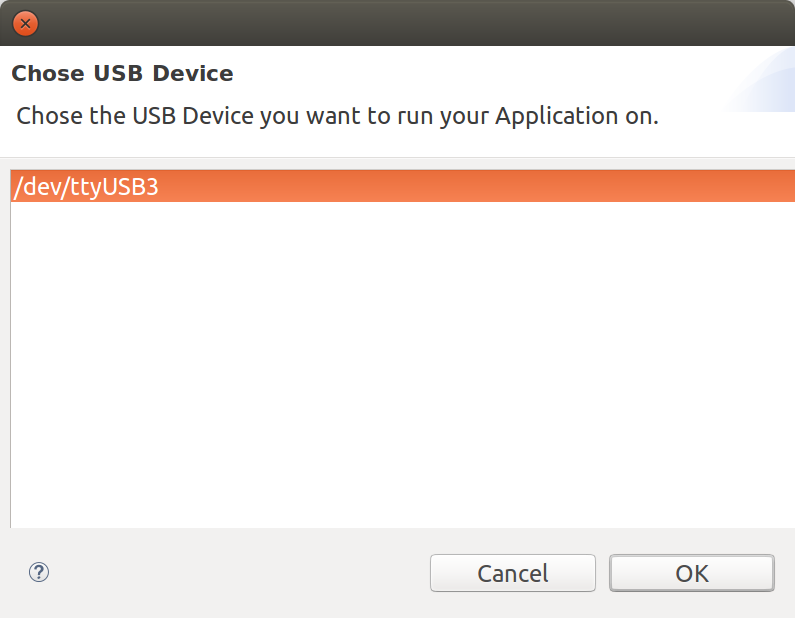
\includegraphics[scale=0.3]{idesettings/umbilical.png}
		\caption{Dialog über welchen der Umbilical Port gesetzt werden kann.}
		\captionsetup{margin=0cm,font={footnotesize}}
		\label{fig:extensionpoint}
\end{figure}

Der Port wird, wenn das Programm ausgeführt wird, automatisch gesetzt. 

\section{Loader}

Der Loader ist das File, welches von gforth mittles dem Befehl:
%
\begin{verbatim}
gforth ./loader.fs
\end{verbatim}
%
gestartet wird. Im Loader befindet sich ein Platzhalter \$INPUT\_FILE, welcher bei der Ausführung des Programms mit dem Namen des Files ersetzt wird.